\documentclass[leqno, 11pt]{article}

\usepackage{lmodern}
\usepackage[scaled]{beramono}
\usepackage[T1]{fontenc}
\usepackage{amssymb}
\usepackage{amsmath}
\usepackage[colorlinks=true]{hyperref}
\usepackage[margin=1in]{geometry}
\usepackage{listings}
\usepackage{graphics}

\graphicspath{/home/brandon/Desktop/IFT_194/labs/photos}

\usepackage{xcolor}
\definecolor{javacommentscolor}{HTML}{646464}
\definecolor{javakeywordscolor}{HTML}{7F0055}
\definecolor{javastringscolor}{HTML}{2A00FF}

\lstset{%
  basicstyle=\footnotesize\ttfamily, % code to be displayed as monospace
  breaklines=true,
  %frame=b
  commentstyle=\color{javacommentscolor},
  keywordstyle=\color{javakeywordscolor},
  stringstyle=\color{javastringscolor},
  showstringspaces=false,  % do not show string spaces character
  tabsize=4,  % change tabs to spaces
  keywordsprefix={@},  % capture method annotations and doctools
  %showtabs=true,
  %tab=|
}

\title{\vspace{6ex}The Java Programming Structure\\
  \Large IFT 194: Lab 1}
\author{Brandon Doyle\\
\href{mailto:bdoyle@asu.edu}{bdoyle5\mbox{}{\fontfamily{ptm}\selectfont @}\mbox{}asu.edu}\\[1em]
Dr. Usha Jagannathan\\
\href{mailto:Usha.Jagannathan@asu.edu}{Usha.Jagannathan\mbox{}{\fontfamily{ptm}\selectfont @}\mbox{}asu.edu}}

\setlength{\parindent}{0em}
\setlength{\parskip}{0.5em}

\begin{document}
\begin{titlepage}
\clearpage\maketitle
\thispagestyle{empty}
\end{titlepage}

\section*{Part A}
I've installed the Java Development Kit (JDK) on my laptop, which is running
Ubuntu 16.04 LTS. We can verify this as follows.
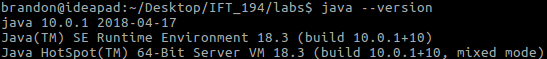
\includegraphics[scale=1.0]{jdk.png}
\section*{Part B}
\subsection*{1 Poem}
\setcounter{subsection}{1}
\subsection{Poem}
Content
\section*{Conclusion}
I spent approximately 5 hours completing this lab. The quickest portion was
setting up my environment as I already had the JDK installed on my Linux 
machine and Eclipse.

Challenges I faced in writing this lab report were primarily around formatting.
Because I've chosen \LaTeX to present my code and findings, 
\newpage
\begin{figure}[t!]
  \centering
  \lstinputlisting[language=java]{/home/brandon/eclipse-workspace/ift_194_labs/src/lab_1/Driver.java}
  \caption{Driver.java}
  \label{fig:one}
\end{figure}

\begin{figure}
  \centering
  \lstinputlisting[language=java]{/home/brandon/eclipse-workspace/ift_194_labs/src/lab_1/Count.java}
  \caption{Count.java}
  \label{fig:two}
\end{figure}

\begin{figure}
  \centering
  \lstinputlisting[language=python]{/home/brandon/projects/visual-inspection-python/example.py}
  \caption{test\_onto.py}
  \label{fig:three}
\end{figure}

\end{document}
